\chapter{Experiments}\label{chp:experiments}

In this chapter the sample implementation is introduced, we'll take a look at the test environment, and present the results.

\section{Test Setup}

Since much of the software to be tested is proprietary and very consumer-oriented, detailed call statistics like dropped packets, latency and bandwidth utilization is not easily available. We need an application-agnostic technique to measure the performance of the different solutions, and our ad-hoc method of doing this is based on comparing timing offsets in the transmitted video stream, and measuring utilized bandwidth as seen by the operating system.

Timing offsets is embedded in the video stream by having each node share their desktop running some pre-recorded video, with an application continously printing a millisecond-accurate clock. Each node can thus find the delay in each stream transmitted to it by finding the difference between it's own clock and the time as transmitted by the other nodes. As long as the clocks on each node is syncronized against the same NTP servers, the clocks should be more than accurate enough to measure the different timing delays observed in the system.

It must be noted, our custom algorithm will not be unjustly favored since it can access the additional forwarding nodes. Google Hangouts and Skype both utilize similar nodes, but their architecture and inner working is hidden from us due to the proprietary nature of these products, and thus they can not be modelled accurately. Only pure peer-to-peer WebRTC products like appear.in and Firefox Hello rely only on the client nodes, but they're both free to add any helpers themselves.


\section{Cost Function}

The cost of utilizing a given network link is a function of the link's utilization, which is given by the classic queuing delay formula, $1/(1 - \mu/\lambda)$. As can be seen in \autoref{fig:utility-latency}, this function is not linear, and can thus not be used directly in our objective function. Nonetheless, we can achieve the same goal -- punishing over-utilization of individual links -- by approximating the function with a piecewise linear graph. The following algorithm partitions a set of slots into a set of edges:

\todo{Insert partitioning-algo here}

Based on this formula, we can formulate the cost multiplier of a link as $1 + k/(\mu - \lambda)$, where $k$ is a customizable parameter for how heavily link saturation should be punished. In our experiments, $k=10$ seems appropriate. This cost function can be seen in \autoref{fig:utility-latency}. We then partion this function into a small set of piecewise linear intervals, which we can model as parallell edges between two nodes, with different capacities and costs. Keeping this set small limits the number of variables in the resulting matrix, and thus keeps processing times reasonably low.

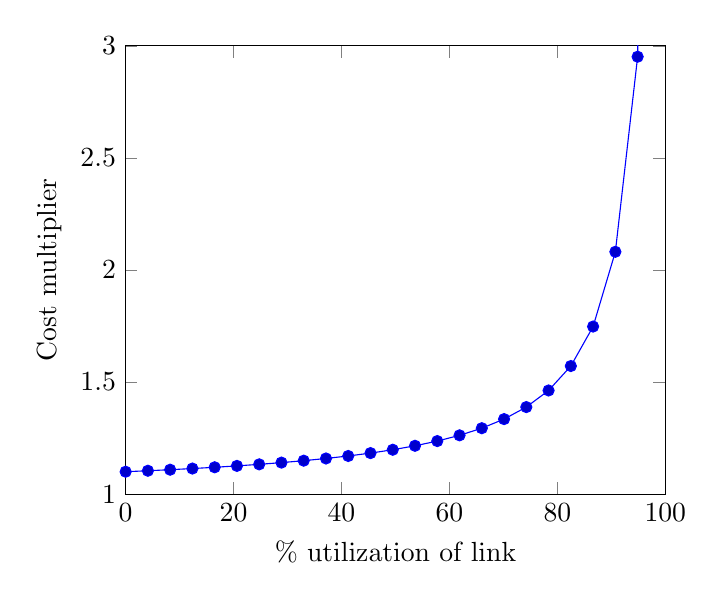
\begin{tikzpicture}
    \begin{axis}[
        xlabel={\% utilization of link},
        ylabel={Cost multiplier},
        xmin=0,
        ymin=1,
        ymax=3,
        xmax=100]

    \addplot+[domain=0:99]{1 + 10/(100 - x)};
    \label{fig:utility-latency}
    \end{axis}
\end{tikzpicture}


\begin{center}
    \label{tab:utilization-to-cost}
    \begin{tabular}{| l | l |}
    \hline
    \textbf{Link utilization} & \textbf{Cost multiplier} \\ \hline
    0--50\% & 1.2 \\ \hline
    51--75\% & 1.40 \\ \hline
    76--80\% & 1.50 \\ \hline
    81--90\% & 2.00 \\ \hline
    \end{tabular}
\end{center}

Using this partitioning as a guide, we can map any number of slots on a physical link into a set of edges $E$ in our graph where $|E| <= 4$.




\section{Implementation}\label{sec:implementation}

\todo{Write about how the implementation was done}


\section{Method}\label{sec:method}

* display latency (can be subtracted)
* display refresh rates (is averaged out (hopefully))
* camera processing times is included in the diff from what's recorded on screen
* chrome devtools echoes browser processing time to be close to ~50ms.

(screensharing scrapped due to framerate artifically limited too severly, did not run any custom code since the solution needed to be (relatively) service agnostic, and could not modify code since it would need to be tagged in the video stream somehow. Some for appear.in, would need to be included in the sdp stream, and extracted -> way too much work).


\section{Results}

To get a sense of how appear.in performs under optimal conditions, a test run was performed with 3, 4 and 7 nodes in a conversation, without any traffic shaping. We would expect both bandwidth and latencies to be fairly even among all the nodes, as the only thing different between them is the time they entered the conversation. Since they were given some time to stabilize before the measurements was started, some fairness should have been achieved.

As we see in \autoref{fig:vanilla-3p}, bitrates between the nodes are identical, as expected. From the latency measurements there seems to be a slight inclination towards the latest arriving node having somewhat higher latencies outgoing, but the difference is negligible in practice.

\begin{figure}
    \centering
    \begin{subfigure}[t]{.48\textwidth}
        \centering
        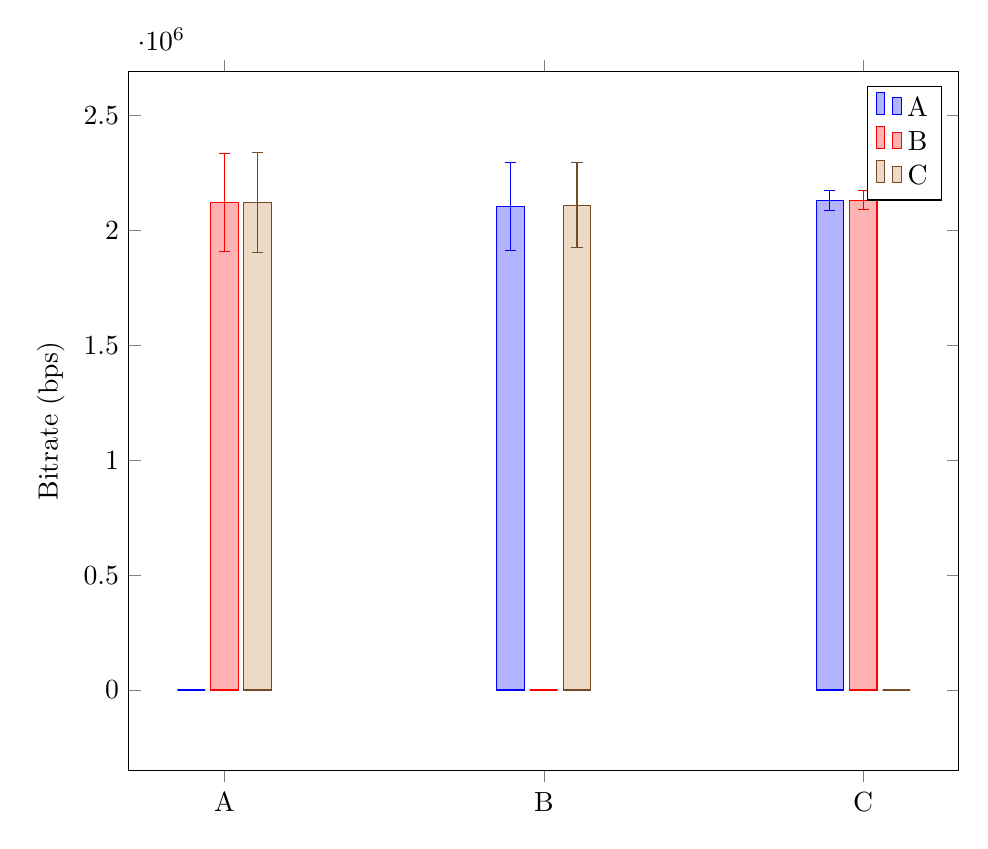
\begin{tikzpicture}
        \begin{axis}[
            ybar,
            ylabel=Bitrate (bps),
            xtick=data,
            width=\textwidth,
            symbolic x coords={A,B,C},
            enlargelimits=0.15
            ]

            %% Traffic received by A
            \addplot+[error bars/.cd,y dir=both, y explicit]
            coordinates{
                (A,0) +- (0.0, 0)
                (B,2103841) +- (0.0, 190915)
                (C,2130058) +- (0.0, 44133)};

            %% Traffic received by B
            \addplot+[error bars/.cd,y dir=both, y explicit]
            coordinates{
                (A,2121908) +- (0.0, 212606)
                (B,0) +- (0.0, 0)
                (C,2130480) +- (0.0, 41317)};

            %% Traffic received by C
            \addplot+[error bars/.cd,y dir=both, y explicit]
            coordinates{
                (A,2121362) +- (0.0, 217821)
                (B,2108437) +- (0.0, 184826)
                (C,0) +- (0.0, 0)};

            \legend{A, B, C}
        \end{axis}
        \end{tikzpicture}
        \subcaption{Outgoing traffic from each node}
    \end{subfigure}
    \hfill
    \begin{subfigure}[t]{.48\textwidth}
        \centering
        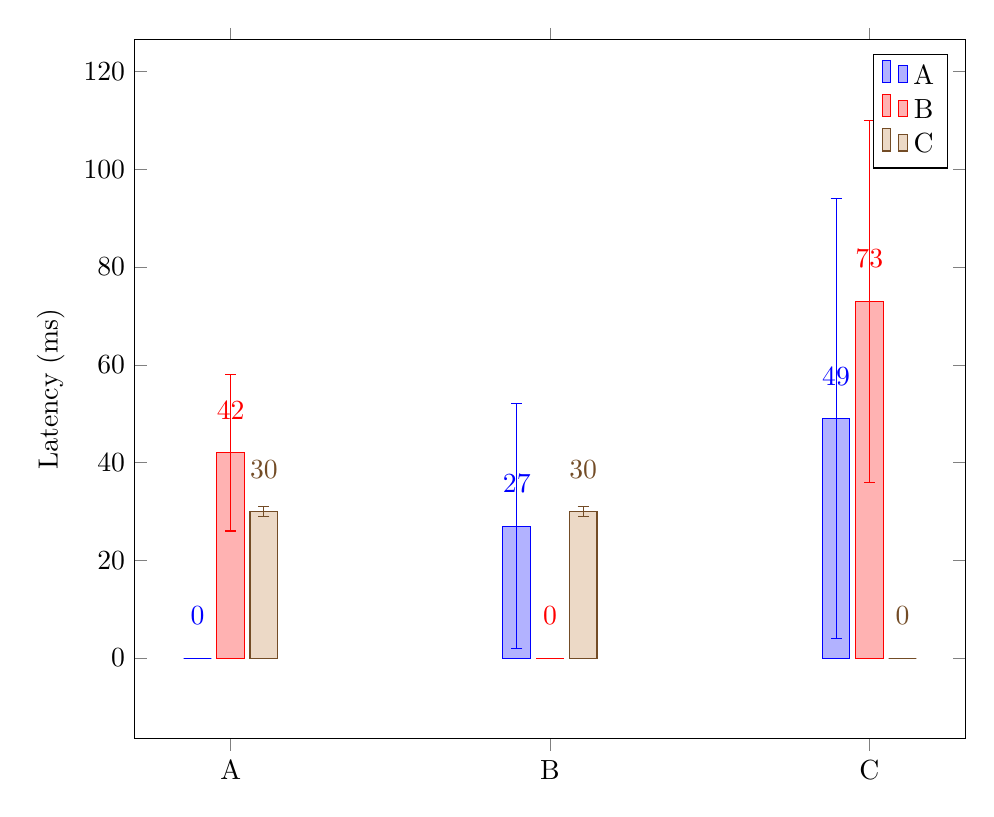
\begin{tikzpicture}
        \begin{axis}[
            ybar,
            compat=newest,
            ylabel=Latency (ms),
            xtick=data,
            width=\textwidth,
            symbolic x coords={A,B,C},
            enlargelimits=0.15,
            nodes near coords=\raisebox{.3cm}{\pgfmathprintnumber{\pgfplotspointmeta}}
            ]

            \addplot+[error bars/.cd,y dir=both, y explicit]
            coordinates{
                (A,0) +- (0.0, 0)
                (B,27) +- (0.0, 25)
                (C,49) +- (0.0, 45)};

            \addplot+[error bars/.cd,y dir=both, y explicit]
            coordinates{
                (A,42) +- (0.0, 16)
                (B,0) +- (0.0, 0)
                (C,73) +- (0.0, 37)};

            \addplot+[error bars/.cd,y dir=both, y explicit]
            coordinates{
                (A,30) +- (0.0, 1)
                (B,30) +- (0.0, 1)
                (C,0) +- (0.0, 0)};

            \legend{A, B, C}
        \end{axis}
        \end{tikzpicture}
        \subcaption{Outgoing latencies for each node}
    \end{subfigure}
    \caption{Test results for three nodes without traffic shaping}
    \label{fig:vanilla-3p}
\end{figure}

Adding another node to the mix, we get the results as shown in \autoref{fig:vanilla-4p}. We see that the bandwidth between the nodes is the same 2.1Mpbs that we saw when there was only three nodes in the conversation, which we can assume is the default transmit bitrate for appear.in. We can also see the same phenomena as in the three node case, that the later arrivals tend to have a slightly higher latency to the nodes first to arrive in the conversation. However, the later nodes (C and D) does not display this phenomena between themselves, thus since all the observations are within one standard deviation of each other we'll not spend any more time investigating this.


\begin{figure}
    \centering
    \begin{subfigure}[t]{.9\textwidth}
        \centering
        \begin{tikzpicture}
        \begin{axis}[
            ybar,
            ylabel=Bitrate (bps),
            xtick=data,
            width=\textwidth,
            bar width=10,
            height=240,
            symbolic x coords={A,B,C,D},
            enlargelimits=0.15
            ]

            %% Traffic received by A
            \addplot+[error bars/.cd,y dir=both, y explicit]
            coordinates{
                (A,0) +- (0.0, 0)
                (B,2108732) +- (0.0, 122299)
                (C,2122345) +- (0.0, 102937)
                (D,2129951) +- (0.0, 31694)};

            %% Traffic received by B
            \addplot+[error bars/.cd,y dir=both, y explicit]
            coordinates{
                (A,2114546) +- (0.0, 77200)
                (B,0) +- (0.0, 0)
                (C,2121893) +- (0.0, 110336)
                (D,2130755) +- (0.0, 31111)};

            %% Traffic received by C
            \addplot+[error bars/.cd,y dir=both, y explicit]
            coordinates{
                (A,2114445) +- (0.0, 61198)
                (B,2109369) +- (0.0, 133375)
                (C,0) +- (0.0, 0)
                (D,2130008) +- (0.0, 32655)};

            %% Traffic received by D
            \addplot+[error bars/.cd,y dir=both, y explicit]
            coordinates{
                (A,2115163) +- (0.0, 72349)
                (B,2108265) +- (0.0, 124281)
                (C,2122517) +- (0.0, 106959)
                (D,0) +- (0.0, 0)};

            \legend{A, B, C, D}
        \end{axis}
        \end{tikzpicture}
        \subcaption{Outgoing traffic from each node}
    \end{subfigure}
    \begin{subfigure}[t]{.9\textwidth}
        \centering
        \begin{tikzpicture}
        \begin{axis}[
            ybar,
            compat=newest,
            ylabel=Latency (ms),
            xtick=data,
            width=\textwidth,
            symbolic x coords={A,B,C,D},
            bar width=10,
            height=240,
            enlargelimits=0.15,
            nodes near coords=\raisebox{.3cm}{\pgfmathprintnumber{\pgfplotspointmeta}}
            ]

            \addplot+[error bars/.cd,y dir=both, y explicit]
            coordinates{
                (A,0) +- (0.0, 0)
                (B,40) +- (0.0, 30)
                (C,60) +- (0.0, 37)
                (D,68) +- (0.0, 25)};

            \addplot+[error bars/.cd,y dir=both, y explicit]
            coordinates{
                (A,51) +- (0.0, 23)
                (B,0) +- (0.0, 0)
                (C,65) +- (0.0, 27)
                (D,65) +- (0.0, 27)};

            \addplot+[error bars/.cd,y dir=both, y explicit]
            coordinates{
                (A,15) +- (0.0, 21)
                (B,15) +- (0.0, 21)
                (C,0) +- (0.0, 0)
                (D,30) +- (0.0, 0)};

            \addplot+[error bars/.cd,y dir=both, y explicit]
            coordinates{
                (A,30) +- (0.0, 27)
                (B,15) +- (0.0, 16)
                (C,37) +- (0.0, 12)
                (D,0) +- (0.0, 0)};

            \legend{A, B, C, D}
        \end{axis}
        \end{tikzpicture}
        \subcaption{Outgoing latencies for each node}
    \end{subfigure}
    \caption{Test results for four nodes without traffic shaping}
    \label{fig:vanilla-4p}
\end{figure}

In the final test without traffic shaping, we step it up to seven nodes in the conversation. The results can be seen in \autoref{fig:vanilla-7p}, and largely mirror what we saw in the smaller experiements. Latencies are a bit higher, which can probably be expected due to the increase in traffic, and apart from a bandwidth deviation on node E, all nodes continue transmitting on the previously observed 2.1Mbps. Why node E's behavior is worse than the other nodes are unknown, but it could be related to node E being on a busier subnet than the other nodes (E was the only node in the test cluster on its subnet).


\begin{figure}
    \centering
    \begin{subfigure}[t]{\textwidth}
        \centering
        \begin{tikzpicture}
        \begin{axis}[
            ybar,
            ylabel=Bitrate (bps),
            xtick=data,
            width=\textwidth,
            bar width=3,
            height=240,
            symbolic x coords={A,B,C,D,E,F,G},
            enlargelimits=0.10
            ]

            %% Traffic received by A
            \addplot+[error bars/.cd,y dir=both, y explicit]
            coordinates{
                (A,0) +- (0.0, 0)
                (B,2130034) +- (0.0, 51733)
                (C,2128127) +- (0.0, 58288)
                (D,2119439) +- (0.0, 153797)
                (E,1516049) +- (0.0, 530232)
                (F,2120354) +- (0.0, 141506)
                (G,2123271) +- (0.0, 92795)};

            %% Traffic received by B
            \addplot+[error bars/.cd,y dir=both, y explicit]
            coordinates{
                (A,2120036) +- (0.0, 154055)
                (B,0) +- (0.0, 0)
                (C,2127250) +- (0.0, 56219)
                (D,2119188) +- (0.0, 160008)
                (E,1453429) +- (0.0, 532842)
                (F,2120152) +- (0.0, 135732)
                (G,2122753) +- (0.0, 90278)};

            %% Traffic received by C
            \addplot+[error bars/.cd,y dir=both, y explicit]
            coordinates{
                (A,2120665) +- (0.0, 150280)
                (B,2130031) +- (0.0, 45591)
                (C,0) +- (0.0, 0)
                (D,2119627) +- (0.0, 152410)
                (E,1543173) +- (0.0, 562049)
                (F,2119490) +- (0.0, 148053)
                (G,2123174) +- (0.0, 96945)};

            %% Traffic received by D
            \addplot+[error bars/.cd,y dir=both, y explicit]
            coordinates{
                (A,2121283) +- (0.0, 153257)
                (B,2128463) +- (0.0, 53731)
                (C,2127889) +- (0.0, 55279)
                (D,0) +- (0.0, 0)
                (E,1676161) +- (0.0, 480970)
                (F,2119602) +- (0.0, 138893)
                (G,2122794) +- (0.0, 89433)};

            %% Traffic received by E
            \addplot+[error bars/.cd,y dir=both, y explicit]
            coordinates{
                (A,2121256) +- (0.0, 153063)
                (B,2130945) +- (0.0, 51320)
                (C,2127847) +- (0.0, 65898)
                (D,2119733) +- (0.0, 158459)
                (E,0) +- (0.0, 0)
                (F,2119668) +- (0.0, 134677)
                (G,2123002) +- (0.0, 95431)};

            %% Traffic received by F
            \addplot+[error bars/.cd,y dir=both, y explicit]
            coordinates{
                (A,2121177) +- (0.0, 151443)
                (B,2132365) +- (0.0, 44058)
                (C,2127846) +- (0.0, 63152)
                (D,2119672) +- (0.0, 153872)
                (E,1094226) +- (0.0, 385404)
                (F,0) +- (0.0, 0)
                (G,2123497) +- (0.0, 96151)};

            %% Traffic received by G
            \addplot+[error bars/.cd,y dir=both, y explicit]
            coordinates{
                (A,2120585) +- (0.0, 155610)
                (B,2132137) +- (0.0, 46317)
                (C,2130083) +- (0.0, 64279)
                (D,2119292) +- (0.0, 154126)
                (E,1602265) +- (0.0, 482579)
                (F,2120748) +- (0.0, 141272)
                (G,0) +- (0.0, 0)};

            \legend{A, B, C, D, E, F, G}
        \end{axis}
        \end{tikzpicture}
        \subcaption{Outgoing traffic from each node}
    \end{subfigure}
    \begin{subfigure}[t]{\textwidth}
        \centering
        \begin{tikzpicture}
        \begin{axis}[
            ybar,
            compat=newest,
            ylabel=Latency (ms),
            xtick=data,
            width=\textwidth,
            symbolic x coords={A,B,C,D,E,F,G},
            bar width=3,
            height=240,
            enlargelimits=0.10,
            nodes near coords=\raisebox{.3cm}{\pgfmathprintnumber{\pgfplotspointmeta}}
            ]

            \addplot+[error bars/.cd,y dir=both, y explicit]
            coordinates{
                (A,0) +- (0.0, 0)
                (B,60) +- (0.0, 31)
                (C,90) +- (0.0, 36)
                (D,88) +- (0.0, 41)
                (E,169) +- (0.0, 29)
                (F,34) +- (0.0, 28)
                (G,47) +- (0.0, 17)};

            \addplot+[error bars/.cd,y dir=both, y explicit]
            coordinates{
                (A,52) +- (0.0, 23)
                (B,0) +- (0.0, 0)
                (C,97) +- (0.0, 52)
                (D,91) +- (0.0, 17)
                (E,144) +- (0.0, 42)
                (F,30) +- (0.0, 18)
                (G,52) +- (0.0, 23)};

            \addplot+[error bars/.cd,y dir=both, y explicit]
            coordinates{
                (A,20) +- (0.0, 17)
                (B,20) +- (0.0, 17)
                (C,0) +- (0.0, 0)
                (D,71) +- (0.0, 18)
                (E,112) +- (0.0, 18)
                (F,20) +- (0.0, 17)
                (G,40) +- (0.0, 17)};

            \addplot+[error bars/.cd,y dir=both, y explicit]
            coordinates{
                (A,22) +- (0.0, 15)
                (B,15) +- (0.0, 17)
                (C,94) +- (0.0, 48)
                (D,0) +- (0.0, 0)
                (E,123) +- (0.0, 24)
                (F,15) +- (0.0, 17)
                (G,15) +- (0.0, 17)};

            \addplot+[error bars/.cd,y dir=both, y explicit]
            coordinates{
                (A,76) +- (0.0, 27)
                (B,86) +- (0.0, 24)
                (C,122) +- (0.0, 34)
                (D,126) +- (0.0, 23)
                (E,0) +- (0.0, 0)
                (F,61) +- (0.0, 19)
                (G,65) +- (0.0, 12)};

            \addplot+[error bars/.cd,y dir=both, y explicit]
            coordinates{
                (A,46) +- (0.0, 17)
                (B,51) +- (0.0, 25)
                (C,102) +- (0.0, 25)
                (D,97) +- (0.0, 23)
                (E,198) +- (0.0, 80)
                (F,0) +- (0.0, 0)
                (G,56) +- (0.0, 12)};

            \addplot+[error bars/.cd,y dir=both, y explicit]
            coordinates{
                (A,47) +- (0.0, 35)
                (B,64) +- (0.0, 24)
                (C,102) +- (0.0, 14)
                (D,95) +- (0.0, 35)
                (E,146) +- (0.0, 33)
                (F,47) +- (0.0, 31)
                (G,0) +- (0.0, 0)};

            \legend{A, B, C, D, E, F, G}
        \end{axis}
        \end{tikzpicture}
        \subcaption{Outgoing latencies for each node}
    \end{subfigure}
    \caption{Test results for seven nodes without traffic shaping}
    \label{fig:vanilla-7p}
\end{figure}




\todo[inline]{[minor] If time, define custom color set for graphing, based possibly either on solarized or http://clrs.cc/}
\todo{Gather some metrics from running the implementation in a prod environment}

For our first test case, "Asia", the bandwidth utilized by each node is shown in \autoref{fig:asia-bitrate}.

\begin{figure}
    \centering
    \begin{subfigure}[t]{.48\textwidth}
        \centering
        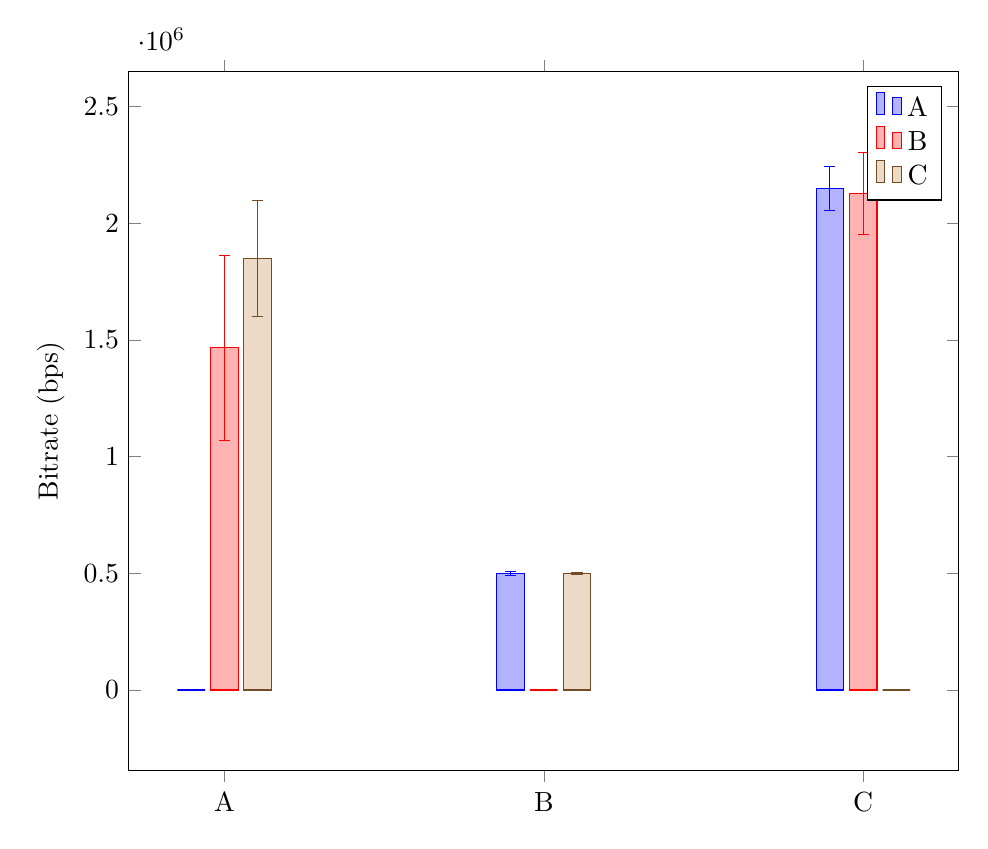
\begin{tikzpicture}
        \begin{axis}[
            ybar,
            ylabel=Bitrate (bps),
            xtick=data,
            width=\textwidth,
            symbolic x coords={A,B,C},
            enlargelimits=0.15
            ]
            %% Traffic received by A
            \addplot+[error bars/.cd,y dir=both, y explicit]
            coordinates{
                (A,0) +- (0.0, 0)
                (B,499012) +- (0.0, 7163)
                (C,2146920) +- (0.0, 94119)};

            %% Traffic received by B
            \addplot+[error bars/.cd,y dir=both, y explicit]
            coordinates{
                (A,1466045) +- (0.0, 396215)
                (B,0) +- (0.0, 0)
                (C,2128002) +- (0.0, 175433)};

            %% Traffic received by C
            \addplot+[error bars/.cd,y dir=both, y explicit]
            coordinates{
                (A,1847944) +- (0.0, 247449)
                (B,498988) +- (0.0, 5709)
                (C,0) +- (0.0, 0)};
            \legend{A, B, C}
        \end{axis}
        \end{tikzpicture}
        \subcaption{Outgoing traffic from each node}
    \end{subfigure}
    \hfill
    \begin{subfigure}[t]{.48\textwidth}
        \centering
        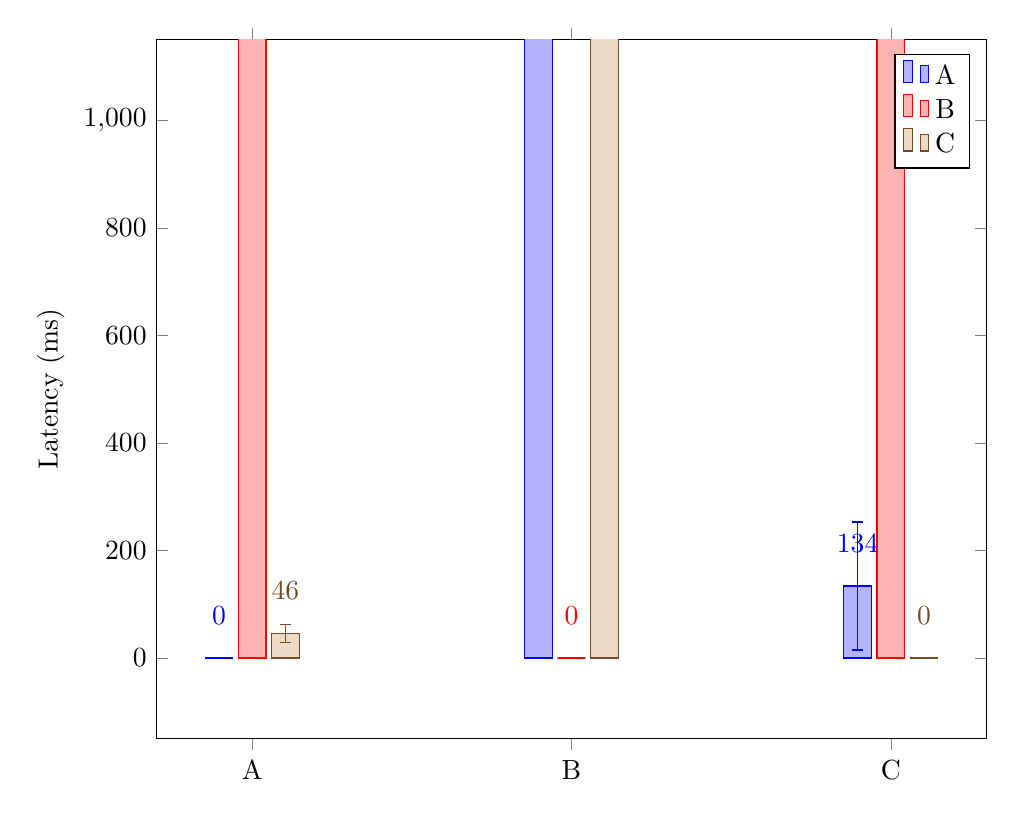
\begin{tikzpicture}
        \begin{axis}[
            ybar,
            compat=newest,
            ylabel=Latency (ms),
            xtick=data,
            ymax=1000,
            width=\textwidth,
            symbolic x coords={A,B,C},
            enlargelimits=0.15,
            nodes near coords=\raisebox{.3cm}{\pgfmathprintnumber{\pgfplotspointmeta}}
            ]

            \addplot+[error bars/.cd,y dir=both, y explicit]
            coordinates{
                (A,0) +- (0.0, 0)
                (B,25186) +- (0.0, 8743)
                (C,134) +- (0.0, 119)};

            \addplot+[error bars/.cd,y dir=both, y explicit]
            coordinates{
                (A,47731) +- (0.0, 23234)
                (B,0) +- (0.0, 0)
                (C,47752) +- (0.0, 23219)};

            \addplot+[error bars/.cd,y dir=both, y explicit]
            coordinates{
                (A,46) +- (0.0, 17)
                (B,24052) +- (0.0, 7647)
                (C,0) +- (0.0, 0)};

            \legend{A, B, C}
        \end{axis}
        \end{tikzpicture}
        \subcaption{Outgoing latencies for each node}
    \end{subfigure}
    \caption{Test results for the "asia" test case.}
    \label{fig:asia-bitrate}
\end{figure}

\begin{figure}
    \centering
    \begin{subfigure}[t]{.9\textwidth}
        \centering
        \begin{tikzpicture}
        \begin{axis}[
            ybar,
            ylabel=Bitrate (bps),
            xtick=data,
            width=\textwidth,
            bar width=10,
            height=240,
            symbolic x coords={A,B,C,D},
            enlargelimits=0.15
            ]
            %% Traffic received by A
            \addplot+[error bars/.cd,y dir=both, y explicit]
            coordinates{
                (A,0) +- (0.0, 0)
                (B,2132647) +- (0.0, 193663)
                (C,1753202) +- (0.0, 229020)
                (D,997887) +- (0.0, 106031)};

            %% Traffic received by B
            \addplot+[error bars/.cd,y dir=both, y explicit]
            coordinates{
                (A,2138074) +- (0.0, 95442)
                (B,0) +- (0.0, 0)
                (C,1938956) +- (0.0, 238021)
                (D,997355) +- (0.0, 103922)};

            %% Traffic received by C
            \addplot+[error bars/.cd,y dir=both, y explicit]
            coordinates{
                (A,2151129) +- (0.0, 116239)
                (B,2068979) +- (0.0, 190976)
                (C,0) +- (0.0, 0)
                (D,999131) +- (0.0, 102965)};

            %% Traffic received by D
            \addplot+[error bars/.cd,y dir=both, y explicit]
            coordinates{
                (A,2161007) +- (0.0, 128042)
                (B,2165180) +- (0.0, 158016)
                (C,2153238) +- (0.0, 218063)
                (D,0) +- (0.0, 0)};
            \legend{A, B, C, D}
        \end{axis}
        \end{tikzpicture}
        \subcaption{Outgoing traffic from each node}
    \end{subfigure}
    \begin{subfigure}[t]{.9\textwidth}
        \centering
        \begin{tikzpicture}
        \begin{axis}[
            ybar,
            ylabel=Latency (ms),
            xtick=data,
            width=\textwidth,
            ymax=1000,
            bar width=10,
            height=240,
            symbolic x coords={A,B,C,D},
            enlargelimits=0.15,
            nodes near coords=\raisebox{.3cm}{\pgfmathprintnumber{\pgfplotspointmeta}}
            ]

            \addplot+[error bars/.cd,y dir=both, y explicit]
            coordinates{
                (A,0) +- (0.0, 0)
                (B,61) +- (0.0, 19)
                (C,252) +- (0.0, 46)
                (D,16168) +- (0.0, 0)};

            \addplot+[error bars/.cd,y dir=both, y explicit]
            coordinates{
                (A,54) +- (0.0, 23)
                (B,0) +- (0.0, 0)
                (C,277) +- (0.0, 27)
                (D,11041) +- (0.0, 0)};

            \addplot+[error bars/.cd,y dir=both, y explicit]
            coordinates{
                (A,140) +- (0.0, 70)
                (B,179) +- (0.0, 71)
                (C,0) +- (0.0, 0)
                (D,15526) +- (0.0, 0)};

            \addplot+[error bars/.cd,y dir=both, y explicit]
            coordinates{
                (A,4683) +- (0.0, 0)
                (B,3437) +- (0.0, 0)
                (C,7750) +- (0.0, 0)
                (D,0) +- (0.0, 0)};

            \legend{A, B, C, D}
        \end{axis}
        \end{tikzpicture}
        \subcaption{Outgoing latencies for each node}
    \end{subfigure}
    \caption{Test results for the "standup" test case.}
\end{figure}


\begin{figure}
    \centering
    \begin{subfigure}[t]{\textwidth}
        \centering
        \begin{tikzpicture}
        \begin{axis}[
            ybar,
            ylabel=Bitrate (bps),
            xtick=data,
            width=\textwidth,
            bar width=3,
            height=240,
            symbolic x coords={A,B,C,D,E,F,G},
            enlargelimits=0.10
            ]

            %% Traffic received by A
            \addplot+[error bars/.cd,y dir=both, y explicit]
            coordinates{
                (A,0) +- (0.0, 0)
                (B,2122914) +- (0.0, 103365)
                (C,1335840) +- (0.0, 353924)
                (D,1433026) +- (0.0, 446130)
                (E,1326235) +- (0.0, 332558)
                (F,1878705) +- (0.0, 235041)
                (G,663701) +- (0.0, 149691)};

            %% Traffic received by B
            \addplot+[error bars/.cd,y dir=both, y explicit]
            coordinates{
                (A,2113784) +- (0.0, 199511)
                (B,0) +- (0.0, 0)
                (C,1313147) +- (0.0, 349341)
                (D,1494177) +- (0.0, 441797)
                (E,1391230) +- (0.0, 311771)
                (F,1971327) +- (0.0, 168470)
                (G,662717) +- (0.0, 190168)};

            %% Traffic received by C
            \addplot+[error bars/.cd,y dir=both, y explicit]
            coordinates{
                (A,2122002) +- (0.0, 198341)
                (B,2130824) +- (0.0, 105922)
                (C,0) +- (0.0, 0)
                (D,1548639) +- (0.0, 413383)
                (E,2031425) +- (0.0, 396762)
                (F,2140084) +- (0.0, 83964)
                (G,661920) +- (0.0, 150000)};

            %% Traffic received by D
            \addplot+[error bars/.cd,y dir=both, y explicit]
            coordinates{
                (A,2128216) +- (0.0, 198663)
                (B,2138372) +- (0.0, 107683)
                (C,1320751) +- (0.0, 360809)
                (D,0) +- (0.0, 0)
                (E,1817435) +- (0.0, 480759)
                (F,2132568) +- (0.0, 82901)
                (G,663245) +- (0.0, 188153)};

            %% Traffic received by E
            \addplot+[error bars/.cd,y dir=both, y explicit]
            coordinates{
                (A,2126240) +- (0.0, 216448)
                (B,2122724) +- (0.0, 139635)
                (C,1283979) +- (0.0, 344558)
                (D,1490125) +- (0.0, 398365)
                (E,0) +- (0.0, 0)
                (F,2125011) +- (0.0, 82898)
                (G,663739) +- (0.0, 148425)};

            %% Traffic received by F
            \addplot+[error bars/.cd,y dir=both, y explicit]
            coordinates{
                (A,1906059) +- (0.0, 236152)
                (B,1902141) +- (0.0, 245489)
                (C,1331865) +- (0.0, 353555)
                (D,1501551) +- (0.0, 438808)
                (E,1925676) +- (0.0, 439134)
                (F,0) +- (0.0, 0)
                (G,663802) +- (0.0, 188379)};

            %% Traffic received by G
            \addplot+[error bars/.cd,y dir=both, y explicit]
            coordinates{
                (A,2125677) +- (0.0, 216945)
                (B,2136130) +- (0.0, 129170)
                (C,1366067) +- (0.0, 330189)
                (D,1513765) +- (0.0, 372789)
                (E,1757906) +- (0.0, 510980)
                (F,2131239) +- (0.0, 93299)
                (G,0) +- (0.0, 0)};

            \legend{A, B, C, D, E, F, G}
        \end{axis}
        \end{tikzpicture}
        \subcaption{Outgoing traffic from each node}
    \end{subfigure}
    \begin{subfigure}[t]{\textwidth}
        \centering
        \begin{tikzpicture}
        \begin{axis}[
            ybar,
            compat=newest,
            ylabel=Latency (ms),
            ymax=1000,
            xtick=data,
            width=\textwidth,
            symbolic x coords={A,B,C,D,E,F,G},
            bar width=3,
            height=240,
            enlargelimits=0.10,
            nodes near coords=\raisebox{.3cm}{\pgfmathprintnumber{\pgfplotspointmeta}}
            ]

            \addplot+[error bars/.cd,y dir=both, y explicit]
            coordinates{
                (A,0) +- (0.0, 0)
                (B,71) +- (0.0, 16)
                (C,9720) +- (0.0, 0)
                (D,5845) +- (0.0, 0)
                (E,341) +- (0.0, 76)
                (F,1329) +- (0.0, 0)
                (G,12792) +- (0.0, 0)};

            \addplot+[error bars/.cd,y dir=both, y explicit]
            coordinates{
                (A,60) +- (0.0, 18)
                (B,0) +- (0.0, 0)
                (C,8163) +- (0.0, 0)
                (D,11178) +- (0.0, 0)
                (E,753) +- (0.0, 1038)
                (F,413) +- (0.0, 404)
                (G,19280) +- (0.0, 0)};

            \addplot+[error bars/.cd,y dir=both, y explicit]
            coordinates{
                (A,12) +- (0.0, 16)
                (B,6) +- (0.0, 13)
                (C,0) +- (0.0, 0)
                (D,9330) +- (0.0, 0)
                (E,2087) +- (0.0, 0)
                (F,2900) +- (0.0, 0)
                (G,27351) +- (0.0, 0)};

            \addplot+[error bars/.cd,y dir=both, y explicit]
            coordinates{
                (A,2074) +- (0.0, 0)
                (B,3056) +- (0.0, 0)
                (C,7300) +- (0.0, 0)
                (D,0) +- (0.0, 0)
                (E,250) +- (0.0, 138)
                (F,36) +- (0.0, 49)
                (G,20225) +- (0.0, 0)};

            \addplot+[error bars/.cd,y dir=both, y explicit]
            coordinates{
                (A,281) +- (0.0, 84)
                (B,1314) +- (0.0, 0)
                (C,9177) +- (0.0, 0)
                (D,10619) +- (0.0, 0)
                (E,0) +- (0.0, 0)
                (F,50038) +- (0.0, 0)
                (G,17236) +- (0.0, 0)};

            \addplot+[error bars/.cd,y dir=both, y explicit]
            coordinates{
                (A,2144) +- (0.0, 0)
                (B,1646) +- (0.0, 0)
                (C,11106) +- (0.0, 0)
                (D,4518) +- (0.0, 0)
                (E,140) +- (0.0, 33)
                (F,0) +- (0.0, 0)
                (G,18154) +- (0.0, 0)};

            \addplot+[error bars/.cd,y dir=both, y explicit]
            coordinates{
                (A,6158) +- (0.0, 0)
                (B,2336) +- (0.0, 0)
                (C,17100) +- (0.0, 0)
                (D,26423) +- (0.0, 0)
                (E,3564) +- (0.0, 0)
                (F,2965) +- (0.0, 0)
                (G,0) +- (0.0, 0)};

            \legend{A, B, C, D, E, F, G}
        \end{axis}
        \end{tikzpicture}
        \subcaption{Outgoing latencies for each node}
    \end{subfigure}
    \caption{Test results for the "friends" test case}
    \label{fig:friends}
\end{figure}
